\documentclass[conference]{IEEEtran}
\IEEEoverridecommandlockouts
% The preceding line is only needed to identify funding in the first footnote. If that is unneeded, please comment it out.
%Template version as of 6/27/2024

\usepackage{cite}
\usepackage{amsmath,amssymb,amsfonts}
% \usepackage{algorithmic}
\usepackage{graphicx}
\usepackage{textcomp}
\usepackage{xcolor}

\usepackage{lineno,hyperref}
\usepackage{minted}
\usepackage{mdframed}

\usepackage{booktabs}
\usepackage{makecell}
\usepackage{subcaption}
\usepackage{float}
\usepackage{multirow}
\usepackage{multicol}
\usepackage{enumitem}

\usepackage{algorithm}  
\usepackage{algorithmicx}  
\usepackage{algpseudocode}

\def\BibTeX{{\rm B\kern-.05em{\sc i\kern-.025em b}\kern-.08em
    T\kern-.1667em\lower.7ex\hbox{E}\kern-.125emX}}

% author center
\makeatletter
\newcommand{\linebreakand}{%
  \end{@IEEEauthorhalign}
  \hfill\mbox{}\par
  \mbox{}\hfill\begin{@IEEEauthorhalign}
}
\makeatother

\begin{document}

\title{COPS: A coroutine-based priority scheduling framework perceived by the operating system}

\author{\IEEEauthorblockN{Anonymous Authors}}

% \author{\IEEEauthorblockN{1\textsuperscript{st} Fangliang Zhao}
% \IEEEauthorblockA{\textit{Tsinghua University} \\
% zfl22@mails.tsinghua.edu.cn}
% \and
% \IEEEauthorblockN{2\textsuperscript{nd} Donghai Liao}
% \IEEEauthorblockA{\textit{Beijing Institute of Technology} \\
% ctrlz.donghai@gmail.com}
% \and
% \IEEEauthorblockN{3\textsuperscript{rd} Jingbang Wu}
% \IEEEauthorblockA{\textit{Beijing Technology and Business University} \\
% wujingbang@btbu.edu.cn}
% \linebreakand
% \IEEEauthorblockN{4\textsuperscript{th} Huimei Lu}
% \IEEEauthorblockA{\textit{Beijing Institute of Technology} \\
% luhuimei@bit.edu.cn}
% \and
% \IEEEauthorblockN{5\textsuperscript{th} Yong Xiang}
% \IEEEauthorblockA{\textit{Tsinghua University} \\
% xyong@tsinghua.edu.cn}  
% }

\maketitle

\begin{abstract}
The multi-threading model in the general operating systems is becoming insufficient in applications with increasing amounts of concurrency, due to the high context-switching costs associated with kernel multi-threading. In this paper, we propose a new concurrency model called COPS. COPS employs a priority-based coroutine model as the fundamental task unit, replacing the traditional multi-threading model in scenarios with high concurrency, and offers a unified priority-based scheduling framework for both kernel and user space coroutines. COPS introduces coroutines as first-class citizens within the OS to provide asynchronous I/O mechanism, using kernel coroutines as a bridge between I/O operations and devices, and user coroutines to bridge applications with the OS services.

We have designed a prototype web server based on COPS and conducted extensive experiments on an FPGA-based system to evaluate COPS. Results show that the proposed model achieves one to four times higher throughput while maintaining relatively lower overhead compared to the multi-threading model in large concurrency applications.
\end{abstract}

\begin{IEEEkeywords}
Multi-threading, Concurrency, Coroutine.
\end{IEEEkeywords}

\section{Introduction}
\label{section: introduction}

In today's era of data explosion, the ability of the general Operating Systems (OS) to process large amounts of data is receiving more attention. For example, Google's servers handle 883 billion requests per day in 2022 \cite{google-search-statistics}, with an average of 8 million requests per second. The increasing scale of the concurrency in the system poses severe challenges to the traditional multi-threading model, which has two main shortcomings in our point of view. First, the multi-threading model is nondeterministic \cite{Lee:EECS-2006-1}. The execution order of threads is uncertain, resulting in the access order of shared resources being uncertain. When used inappropriately in fixed workflows, multi-threading can lead to greater overhead. In order to improve the performance of the multi-threading model in large concurrency scenarios such as the web server, some research has tried to optimize it, but has not solved the problem mechanically \cite{li_combining_2007, howell_cooperative_2002}.

Second, the multi-threading model is incompatible with the asynchronous I/O mechanism in OS. For instance, Linux employs an event-driven model, such as \textit{select} and \textit{epoll} to handle multiple I/O operations on a single thread, involving producer-consumer interaction and increasing the cost of synchronous mutual exclusion, thereby adding to the kernel's complexity \cite{Gammo2004ComparingAE}. Similarly, Windows' I/O Completion Ports(IOCP) \cite{alvinashcraft_io_2022} offers I/O multiplexing but can be challenging to program correctly due to callback functions \cite{callbackhell}. The io\_uring model, introduced in \cite{io_uring}, enhances both efficiency and throughput by leveraging shared memory to eliminate data copying. However, this approach adds kernel complexity and complicates interface usage \cite{li2021pm}. Furthermore, because the OS lacks awareness userland asynchronous tasks, asynchronous interfaces implemented in userland, such as POSIX AIO, result in increased overhead due to thread management, I/O buffer replication, and context switching across privilege levels \cite{jones2006boost}.

Asynchronous I/O mechanisms are effective in high concurrency web server environments but pose significant design and implementation challenges. The challenges arise not only from enabling asynchronous I/O for applications within kernel but also from developing runtime environment for kernel's asynchronous tasks. LXDs \cite{narayanan2019lxds} created an in-kernel asynchronous runtime for efficient cross-domain processing. Memif \cite{lin2016memif} offered a low-latency, low-overhead interface using asynchronous and hardware-accelerated techniques. Lee \textit{et al.} \cite{lee2019asynchronous} introduced the asynchronous I/O stack (AIOS) to the kernel to reduce the I/O latency. Despite these advancements, most methods function independently of the kernel's thread scheduler, which limits their adaptability and scalability and further complicates the kernel's design.

As an alternative concurrency model, the concept of coroutines has not been widely adopted in modern programming languages in many decades. Currently, there is a renewal of interest in coroutines to explore their advantages as an alternative to multi-threading. In this paper, we rethink the concurrency model and asynchronous framework to find solutions that could meet the larger-scale and higher performance requirements. We propose COPS\footnote{The \textbf{CO} in COPS represents the coroutine, \textbf{P} represents the priority, and \textbf{S} represents scheduling. All tasks must be carried out under COPS's management.}, a coroutine-based priority scheduling framework in OS. COPS improves high context-switching overhead and solve the problem of uncertain sequence of accessing shared resources by using coroutines as the fundamental task unit. In addition, COPS builds upon existing research on asynchronous I/O mechanisms, integrates coroutines within the kernel, treats them as first-class citizens, and combines them with the asynchronous I/O mechanism to provide a coordinated and unified scheduling framework for all tasks within the OS.

The rest of the paper is organized as follows: In Section \ref{section: Background}, we explain the fall and resurgence of coroutines and the coroutine facilities in Rust language. Section \ref{section: design} details the design of COPS, while Section \ref{section: Common usage patterns} explores common patterns in asynchronous and concurrent programming. Performance results for COPS are presented in Section \ref{section: Performance Evaluation}. We review related work in Section \ref{section: Related Work} and conclude in Section \ref{section: Conclusion}.

\section{Background}
\label{section: Background}

\subsection{Coroutine}

Coroutines, introduced in the 1960s, offer a lightweight way to improve concurrency with lower resources and overheads compared to processes or threads. The core characteristics of coroutines, shown as follows, are summarized in \cite{1980Coroutines}:

\begin{itemize}[leftmargin=*]
  \item[1)] The values of data local to a coroutine persist between successive calls;
  \item[2)] The execution of a coroutine is suspended as control leaves it, only to carry on where it left off when control re-enters the coroutine at some later stage.
\end{itemize}

However, this general definition leaves open relevant issues regarding the coroutine construct, affecting how coroutine facilities are supported in programming languages. Misunderstandings about the expressive power of coroutines have been perpetuated by some implementations. Additionally, the introduction of first-class continuations and the adoption of multi-threading as a "de facto standard" for concurrent programming have led to a decline in the use of coroutines.

The revival of coroutines stems from the fact that Moura et al. \cite{2009Revisiting} have demonstrated that full coroutines have an expressive power equivalent to one-shot continuations and one-shot delimited continuations. Nowdays, modern programming languages, c++ 20 \cite{C++20-coroutine}, Go \cite{goroutines}, Rust \cite{rosendahl2017green}, Python \cite{python-coroutine}, Kotlin \cite{kotlin-coroutines}, etc., all provide varying degrees of support for coroutines.

\subsection{The Coroutine facilities in Rust}
\label{subsection: rust_async}

Rust, a modern language, excels in performance, security, and concurrency. It features a robust trait system that offers similar capabilities as object-oriented languages, including abstraction, inheritance, and polymorphism.

In Rust, the coroutine facilities is based on its trait system. Rust provides a special trait named \textbf{Future} in its core library. Any object that implements \textbf{Future} exhibits asynchronous, which is called as coroutines. The poll method defined by the Future trait advances the coroutine's execution. If poll returns Poll::Ready, it indicates the coroutine has completed. Returning Poll::Pending signifies the coroutine is awaiting an event before resuming. The Future trait is detailed in listing \ref{future_trait}.

\begin{listing}[tbp]
\caption{Future trait.}
\label{future_trait}
\begin{mdframed}
\begin{minted}[linenos=false,breaklines]{rust}
pub trait Future {
  type Output;
  fn poll(self: Pin<&mut Self>, cx: &mut Context<'_>) -> Poll<Self::Output>;
}
enum Poll<T> {
  Ready(T),
  Pending,
}
\end{minted}
\end{mdframed}
\end{listing}

Besides manually implementing Future trait, Rust provides async/await keywords for creating and executing coroutines. The async keyword converts functions, blocks, or closures into futures without explicitly implementing the Future trait. The await keyword executes Future objects and, when an operation cannot continue, relinquishes the CPU.

Through the Future trait and async/await keywords in Rust, coroutines are treated as first-class citizens for developers at the language level. Moreover, Rust separates the coroutine runtime from the definition of coroutines, enabling customization of runtimes. This separation and the flexibility in definition could pave the way for introducing coroutines at the kernel level, beyond just user space, and even making coroutines as first-class citizens at the OS level.

\section{Design of COPS}
\label{section: design}

COPS is designed to enhance system concurrency by treating coroutines as the fundamental task unit and integrating them as first-class citizens within the OS. COPS offers a unified priority-based scheduling system for coroutines in both kernel and user spaces, enabling both kernel and application developers to freely utilize coroutines. Fig.\ref{fig:arch} illustrates COPS's overall structure. Both applications and the OS maintain their own Executor data structures and share COPS's scheduling framework via vDSO \cite{michael_kerrisk_vdso7_2023}. They represent tasks as coroutines and manage tasks by using COPS's services through function calls. Applications access other system services via system calls. Additionally, the OS maintains a global bitmap for advanced priority-based cooperative scheduling.

\begin{figure}[tbp]
  \centering
  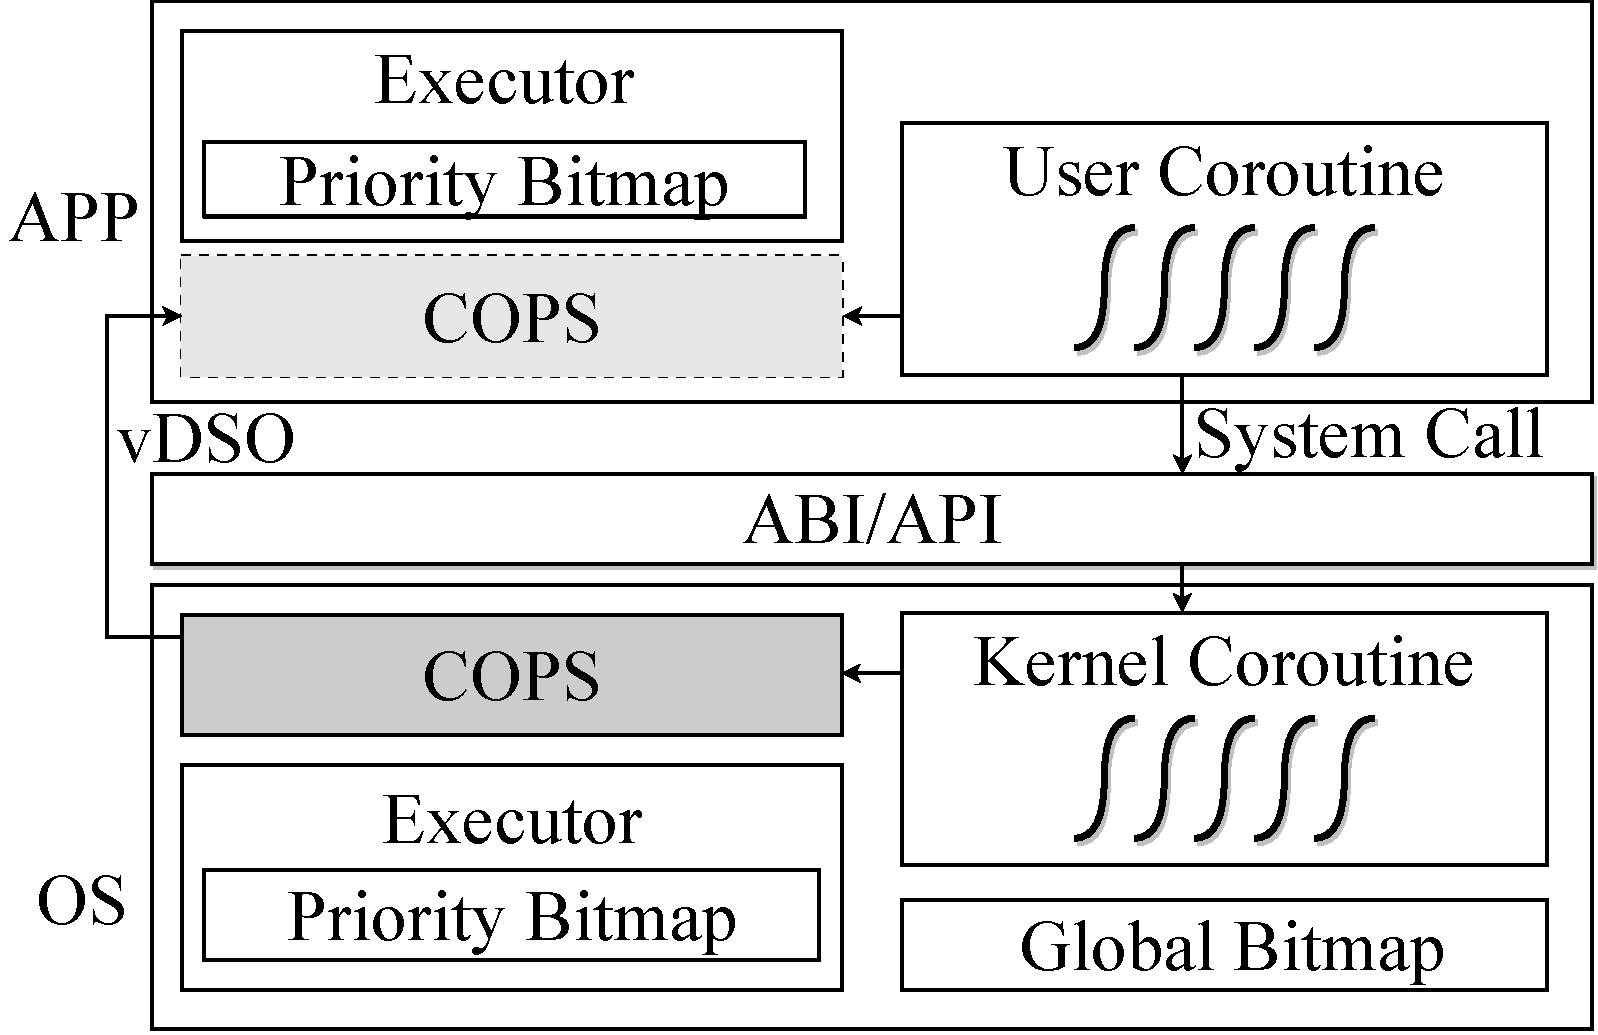
\includegraphics[width=\linewidth]{assets/arch.pdf}
  \caption{The architecture of COPS.}
  \label{fig:arch}
  \vspace{-1em}
\end{figure}

In this section, we detail the design of COPS. We start by explaining the data structures behind COPS's coroutine runtime and how they enable coroutine scheduling (\ref{section: Coroutine Runtime}). We then discuss the coroutine state transition model (\ref{section: state-transition}). Following that, we outline the COPS API (\ref{section: cops api}). Lastly, we describe COPS's global cooperative scheduling mechanism (\ref{section: global-cooperative-scheduling}).

\subsection{Coroutine Runtime}
\label{section: Coroutine Runtime}

Rust offers the \textbf{Future} and \textbf{Wake} traits to facilitate coroutines without tying them to a specific runtime. This flexibility facilitates the creation of a coroutine runtime suitable for both kernel and user space. The runtime consists of two main components: 

\subsubsection{Coroutine Control Block}

As detailed in \ref{subsection: rust_async}, the poll method in Future trait is partially transparent, limiting the precise control of coroutines. To address this, we extends Rust's future and wake abstractions to create coroutine control blocks (CCBs) for more precise control. The CCB structure is displayed in listing \ref{ccb}. The Wake trait is responsible for saving and restoring coroutine contexts. Both the execution and the context-switching of the coroutine are done by the compiler and are transparent. Therefore, the future and wake must be described in the CCB. However, relying solely on the future and wake traits results in a basic polling mechanism that cannot allow for precise control or integration with asynchronous I/O. To enable precise control, we have enhanced the CCB with three additional fields: 1) The Cid is used to identify CCB, and plays a key role in asynchronous I/O mechanism; 2) The Kind denotes the type of the coroutine, guilding the subsequent processing after the coroutine reaches a certain stage; 3) The Priority reflects the coroutine's priority level, which is fundamental to COPS's scheduling framework. The state field is not included in the CCB because Rust coroutines only exist in pending or ready states, with their state implicitly indicated by the queue they reside in.


\begin{listing}
\caption{Coroutine control block.}
\label{ccb}
\begin{mdframed}
\begin{minted}[linenos=false,breaklines]{rust}
pub struct Coroutine{
  pub cid: CoroutineId,
  pub kind: CoroutineKind,
  pub priority: usize,
  pub future: Pin<Box<dyn Future<Output=()> + 'static + Send + Sync>>, 
  pub waker: Arc<Waker>,
}
\end{minted}
\end{mdframed}
\end{listing}

\subsubsection{Executor}
\label{subsubsection: executor}

The core of the coroutine runtime is the Executor, which manages all coroutines in a process based on the coroutine control block. The Executor's primary components consist of the following:

\begin{itemize}[leftmargin=*]
    \item[1)] Ready Queues and Priority Bitmaps: The Executor manages queues of coroutines sorted by priority, ensuring that the highest priority coroutine is always executed first. It also employs a priority bitmap to track the presence of coroutines at each priority level. This bitmap, while not needed for user-level Executors, aids in OS-level scheduling by providing the OS with visibility into user-level coroutines.
    \item[2)] Blocking Set: This structure manages all coroutines that are blocked, holding them until the awaited event occurs and triggers their resumption.
\end{itemize}

These two data structures form the runtime foundation for coroutines and establish a basic priority scheduling mechanism for COPS. This ensures that within a address space, COPS can effectively prioritize and schedule the highest-priority coroutine each time.

\subsection{Coroutine State Transition Model}
\label{section: state-transition}

Treating coroutines as first-class citizens within the OS has transformed traditional process and thread concepts. For instance, under Kernel Page Table Isolation(KPTI) \cite{kpti}, the kernel acts as a special process with address space switches upon entry and return. Threads now act as stack providers for coroutines and provide abstractions for multiprocessor systems, rather than being the primary unit of scheduling.

The traditional thread state model has been supplanted by the coroutine state model, which includes five basic states: create, ready, running, blocked, and exit, plus a special running-suspended state due to preemptive scheduling and other interruptions. When a coroutine's execution is interrupted by a timer interrupt, exceptions, or synchronous system calls, it occupies the stack but does not actively execute on the CPU, hence the term "running-suspended." This can be further categorized into interrupt and exception sub-states. The coroutine state transition model is depicted in Fig.\ref{fig:state}.

\begin{figure}[tbp]
  \centering
  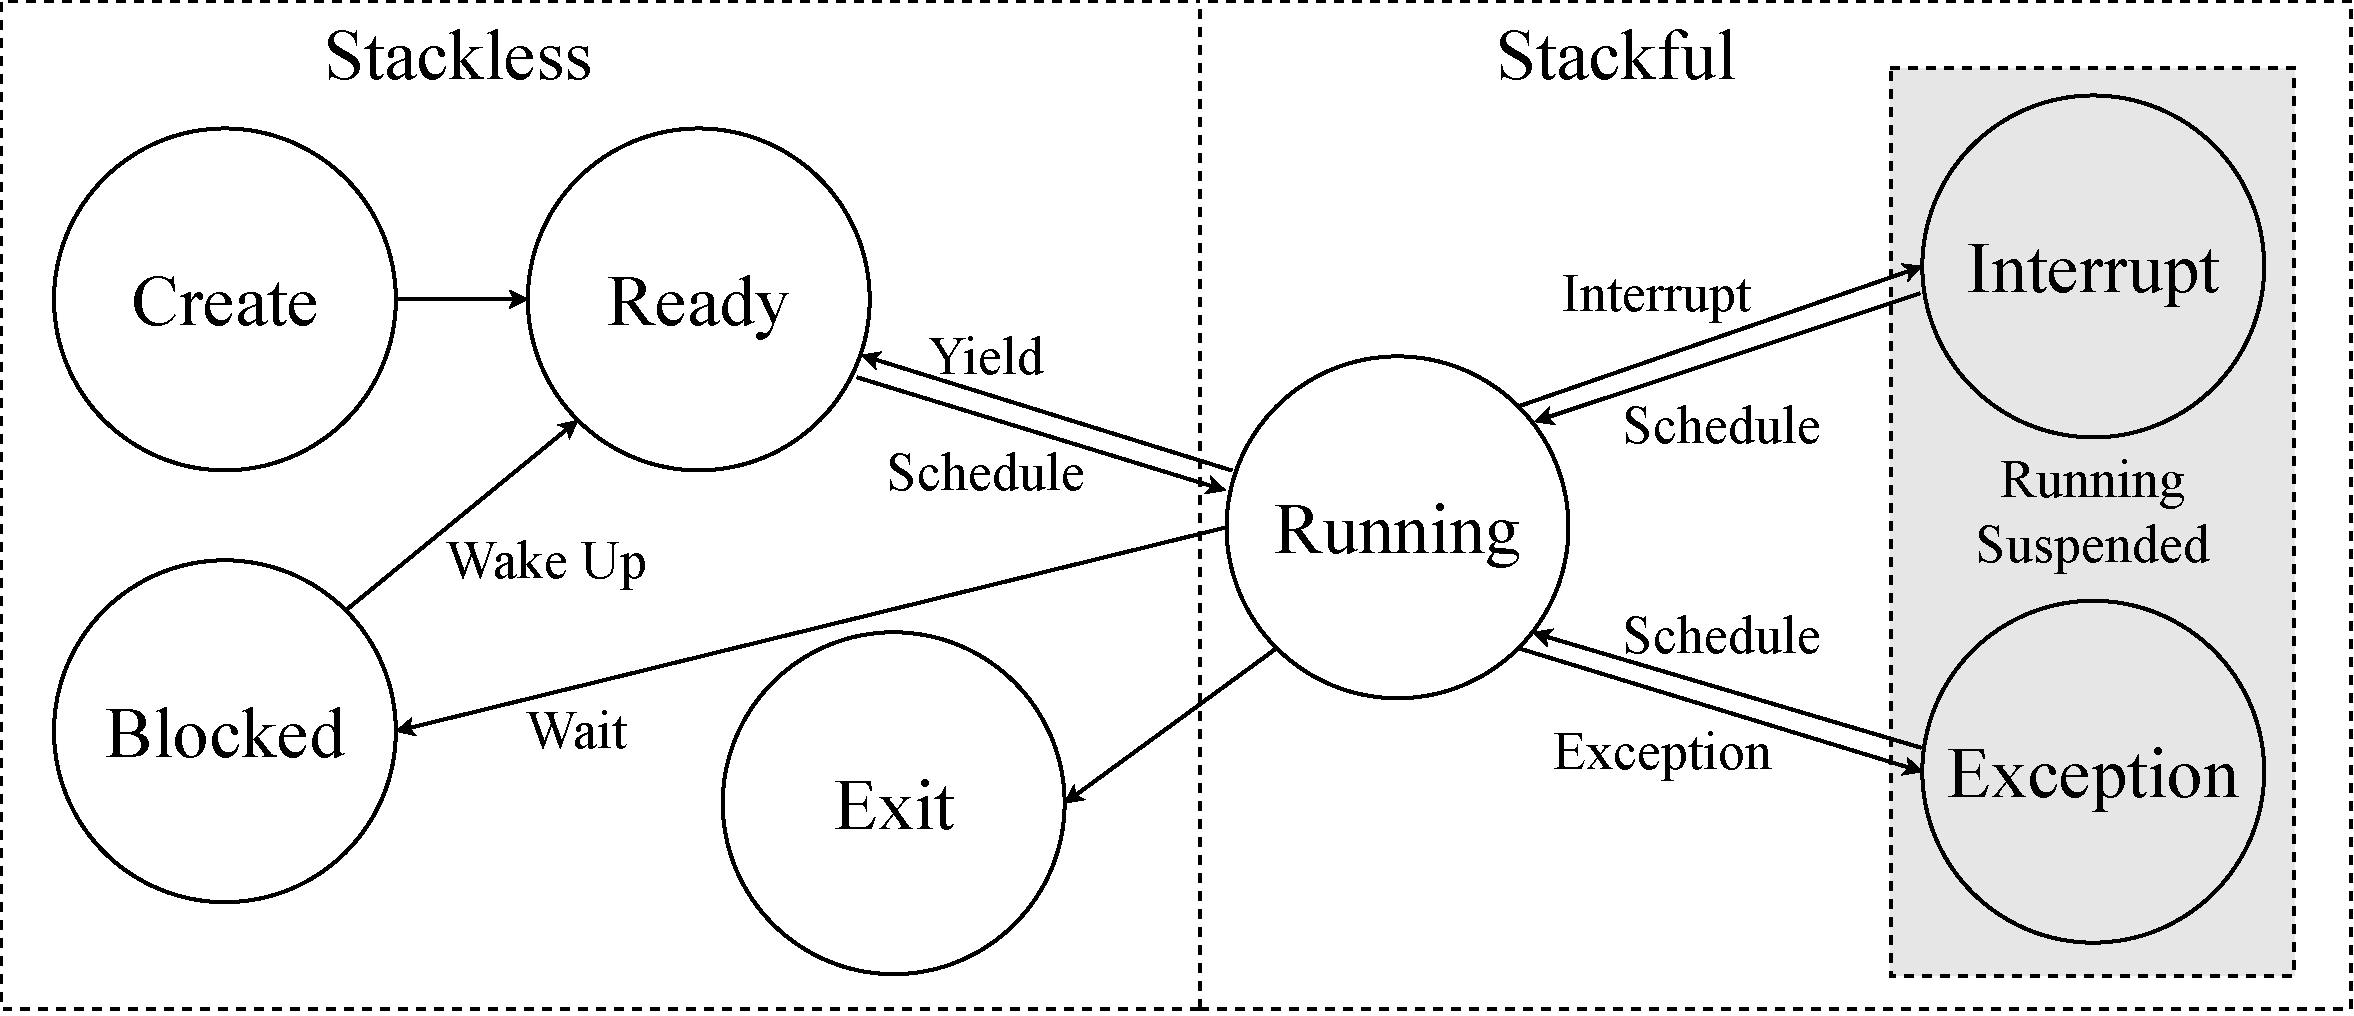
\includegraphics[width=\linewidth]{assets/cstate.pdf}
  \caption{Coroutine state transition model.}
  \label{fig:state}
  \vspace{-1em}
\end{figure}

\begin{enumerate}[leftmargin=*]
    \item When a coroutine is created, it begins in the ready state and moves to the running state once it is scheduled.
    \item A running coroutine can either wait for an event and enter the blocked state, or yield to higher-priority coroutines and become ready again. This transition does not utilize the coroutine's execution stack. Alternatively, if an interrupt or exception occurs, the coroutine enters a suspended state. Upon task completion, it transitions to the exit state, where resource cleanup is performed.
    \item In the blocked state, a coroutine awaits an event to transition back to the ready state. If it is in a suspended state, it bypasses the ready state and waits for the completion of the relevant handling routine before resuming execution.
\end{enumerate}

\subsection{COPS API}
\label{section: cops api}

Coroutines typically have three basic operations: \textit{create}, \textit{resume} and \textit{yield}. In Rust, the \textit{resume} and \textit{yield} operators are replaced by the poll function and the await keyword respectively.
Since the future must be driven by await keyword, it is not necessary to consider whether the \textit{yield} is placed correctly within the asynchronous tasks. However, developers must be careful using loop to avoid occupying the CPU for a long time. It is worth mentioning that COPS addresses the issue of accidentally using tight loops by employing a global cooperative scheduling mechanism, detailed in section \ref{section: global-cooperative-scheduling}.

COPS offers a \textit{spawn} function to create new coroutines, along with additional APIs (\textit{current, wake\_up, set\_priority, alloc\_cpu}) to enhance the control of coroutines. The \textit{spawn} initiates a coroutine and returns its identity, the \textit{current} retrieves the identity of the current coroutine, the \textit{wake\_up} revives a specified coroutine, the \textit{set\_priority} adjusts a coroutine's priority, and \textit{alloc\_cpu} requests additional CPU resources. By default, applications are allocated one CPU, but \textit{alloc\_cpu(1)} can be used to request more. Table \ref{tab:interface} lists the COPS APIs.

With the COPS API, developers can fully leverage coroutines in both kernel and user space with minimal restrictions.

\begin{table}[htbp]
  \centering
  \begin{tabular}{@{}cc@{}}
  \toprule
  Function                     & Return Value \\ \midrule
  spawn(future, priority)      & cid          \\
  current()                    & cid          \\
  wake\_up(cid)                &              \\
  set\_priority(cid, priority) &              \\
  alloc\_cpu(cpu\_num)          &              \\ \bottomrule
  \end{tabular}
  \caption{Interface of COPS.}
  \label{tab:interface}
  \vspace{-1em}
\end{table}

\subsection{Global Cooperative Scheduling Mechanism}
\label{section: global-cooperative-scheduling}

COPS offers an advanced global cooperative scheduling mechanism that includes both between kernel and user process and between user process. The priority bitmap, as described in \ref{subsubsection: executor}, is crucial for this mechanism.

COPS facilitates coordination between kernel and user process coroutines through a global cooperative scheduling approach. Upon the timer interrupt, the kernel scans the priority bitmaps of user process Executors to construct a global priority bitmap, thereby giving the OS awareness of user-level coroutines. Additionally, the kernel possesses an Executor for managing its own coroutines.

COPS integrates coroutine and process scheduling within the kernel. One approach is to have distinct schedulers for processes and coroutines, prioritizing kernel coroutines over user processes. However, this approach can complicate the system and not fully address kernel asynchronous I/O issues discussed in \ref{section: introduction}. A more elegant solution involves a special \textbf{switching coroutine} in the kernel that identifies the highest-priority user process, manages switching operations, and persists as long as user processes exist. It matches the highest process priority, ensuring cooperative scheduling between the kernel and user processes based on their priorities. The kernel statically assigns the \textbf{switching coroutine} the highest priority at initialization, with dynamic adjustments made during runtime based on priority bitmap scans. This allows the kernel to reuse COPS's priority scheduling mechanism for both process and coroutine scheduling. If the kernel has higher-priority coroutines, all user process coroutines are considered of lower priority and wait for the kernel coroutines to complete execution. The \textbf{switching coroutine} can then schedule the highest-priority process, coordinating between kernel coroutines and user processes.

Furthermore, COPS provide user processes with read-only access to the global priority bitmap, for coordinating coroutines across various processes. If a user process detects a higher-priority coroutine within the kernel or other processes, it will proactively yield to facilitate cooperative multitasking. However, excessive global coordination might lead to issues such as prolonged CPU usage by malicious processes or high switching overhead, which we aim to address in our future research. These concerns, while important, are beyond the scope of the present paper.

This mechanism allows COPS to offer an OS-aware coroutine scheduling framework that prevents any single coroutine from monopolizing CPU resources for extended periods. Fig.\ref{fig:flow} illustrates the code logic of COPS.

\begin{figure}[tbp]
  \centering
  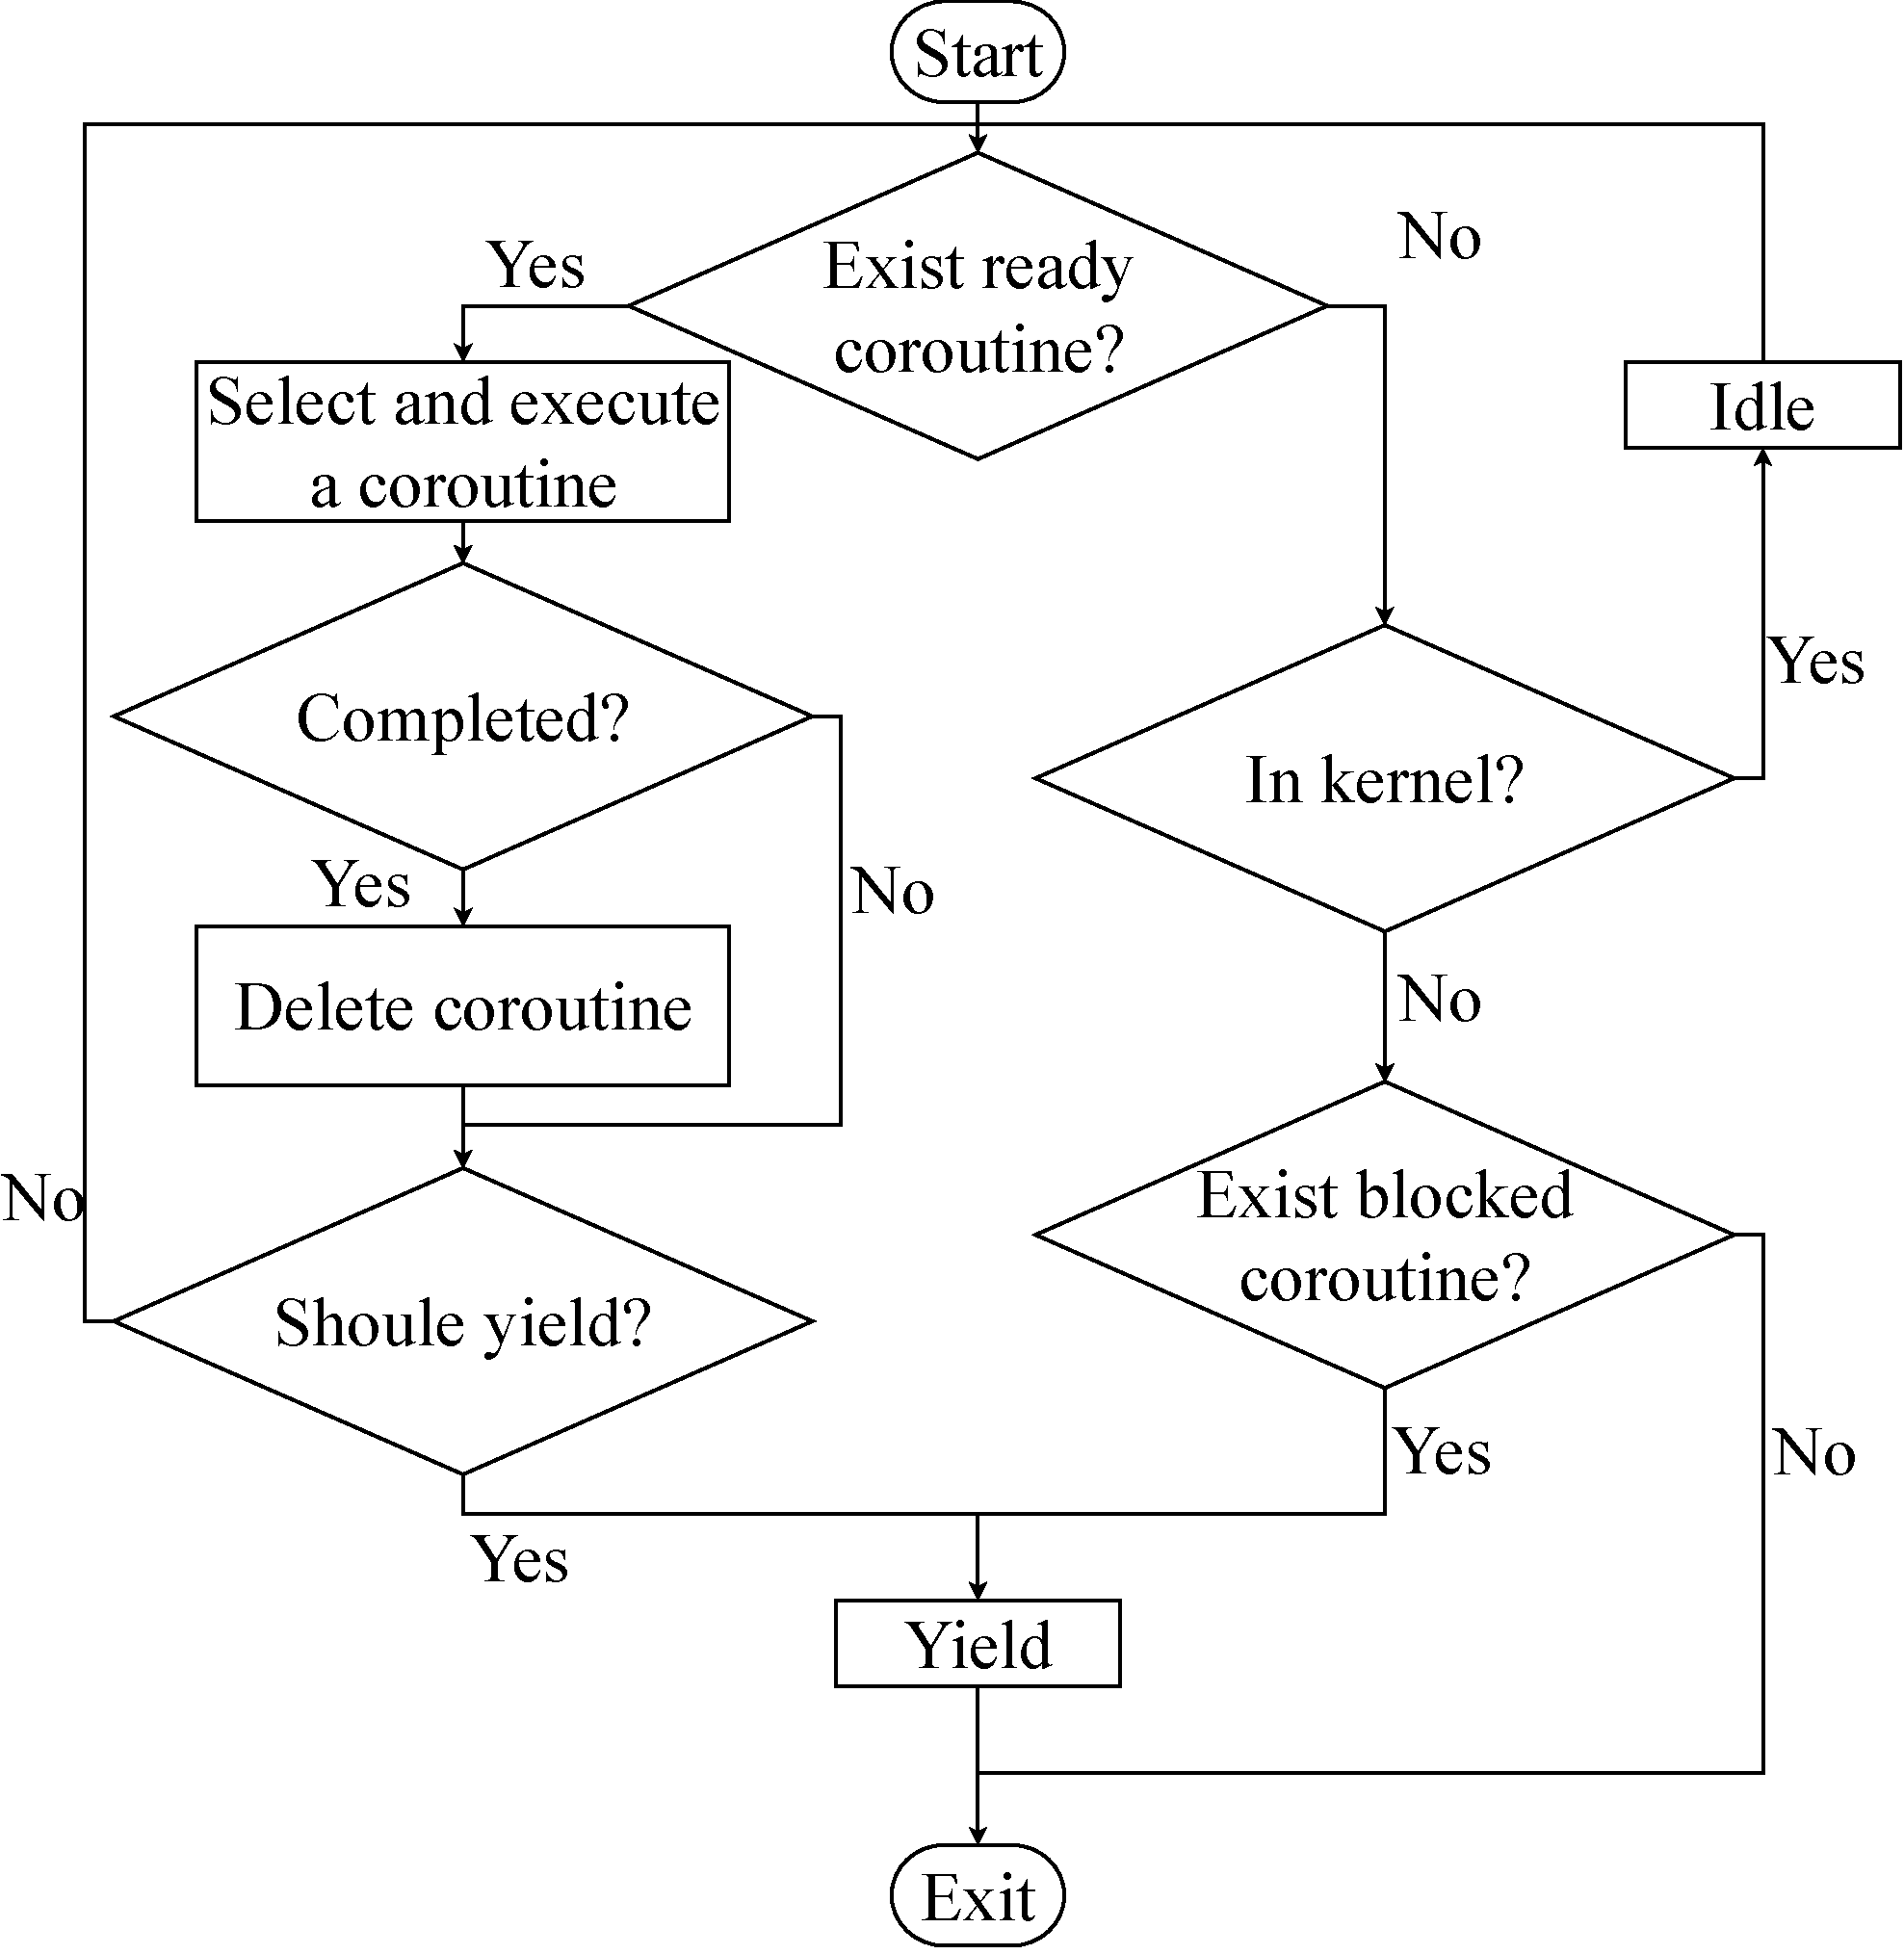
\includegraphics[width=\linewidth]{assets/flow.pdf}
  \caption{The code logic of COPS.}
  \label{fig:flow}
  \vspace{-1em}
\end{figure}

\section{Common usage patterns}
\label{section: Common usage patterns}

In this section, we demonstrate concurrent and asynchronous programming patterns using COPS. COPS creates an environment where all tasks are executed as coroutines. The application's main task is to use the \textit{spawn} function to initiate coroutines for specific tasks. The execution of these coroutines is automatically managed by COPS's coroutine runtime, operating transparently.

\subsection{Concurrency}

A typical COPS use pattern is depicted in Algorithm \ref{alg: concurrency}, where the application initiates two coroutines: a producer and a consumer. The producer generates data and, when the message queue is full, signals the consumer and yields the CPU. The consumer then processes all data and waits. Subsequently, COPS reschedules the producer.

\begin{algorithm}[!ht]
  \caption{Concurrent Programming}
  \label{alg: concurrency}
  \begin{algorithmic}[1]
    \State $MSG\_QUEUE;$
    \Function{main}{}
      \State $consumer\_cid \gets spawn(|| consumer, 1)$;
      \State $spawn(|| producer(consumer\_cid), 0)$;
		\EndFunction

    \Function{consumer}{}
      \Loop
        \While{MSG\_QUEUE is empty}
          \State blocked;
        \EndWhile
        \State ... \Comment{consume data from MSG\_QUEUE}
      \EndLoop
    \EndFunction

    \Function{producer}{cid}
      \Loop
        \While{MSG\_QUEUE is full}
          \State wake\_up(cid); \Comment{wake up the consumer}
          \State yield;
        \EndWhile
        \State ... \Comment{produce data into MSG\_QUEUE}
      \EndLoop
    \EndFunction
  \end{algorithmic}
\end{algorithm}

\subsection{Asynchronous Programming}

Another common COPS pattern is for asynchronous programming. By leveraging COPS's coroutine runtime environment, we can convert synchronous system calls into asynchronous ones using coroutines. However, simply changing the interface is not sufficient; the kernel must also implement support for these asynchronous system calls.

\begin{itemize}[leftmargin=*]
  \item[1)] System Call Interfaces: We have introduced an \textbf{Asyncall} data structure that implements Rust's Future trait to handle system calls asynchronously. This structure checks the return values of system calls to determine whether asynchronous waits are required. Rust macros ensure a consistent format for both synchronous and asynchronous system calls, with the latter requiring an additional parameter. An example is shown in the read system call interface \ref{listing: system call}.
  \item[2)] Kernel Asynchronous I/O Support: When a user coroutine initiates an asynchronous system call, the kernel creates a corresponding kernel coroutine that is not executed immediately. Control promptly returns to the user coroutine, allowing it to pause while enabling other user coroutines to run. Once the kernel coroutine completes the asynchronous operation, it awakens the related user coroutine using the cid provided by the system call.
\end{itemize}

Algorithm \ref{alg: asynchronous programming} illustrates asynchronous programming using the asynchronous system call interface. In the async\_read function, it initiates an asynchronous \textit{read!} system call. If the kernel buffer is empty, async\_read yields the CPU. When data becomes available in the kernel buffer, async\_read is awakened to continue execution.

\begin{algorithm}[!ht]
  \caption{Asynchronous Programming}
  \label{alg: asynchronous programming}
  \begin{algorithmic}[1]
    \Function{main}{}
      \State $spawn(|| async\_read, 0)$;
		\EndFunction

    \Function{async\_read}{}
      \State $buf \gets [0; buf\_len]$;
      \State $current\_cid \gets current()$;
      \State $read!(buf.ptr, buf.len, current\_cid)$;
    \EndFunction
  \end{algorithmic}
\end{algorithm}

\begin{listing}
  \caption{System call interface of read().}
  \label{listing: system call}
  \begin{mdframed}
  \begin{minted}[linenos=false,breaklines]{rust}
  read!(fd, buffer, cid); // Async
  read!(fd, buffer); // Sync
  \end{minted}
  \end{mdframed}
\end{listing}

\begin{figure}[tbp]
  \centering
  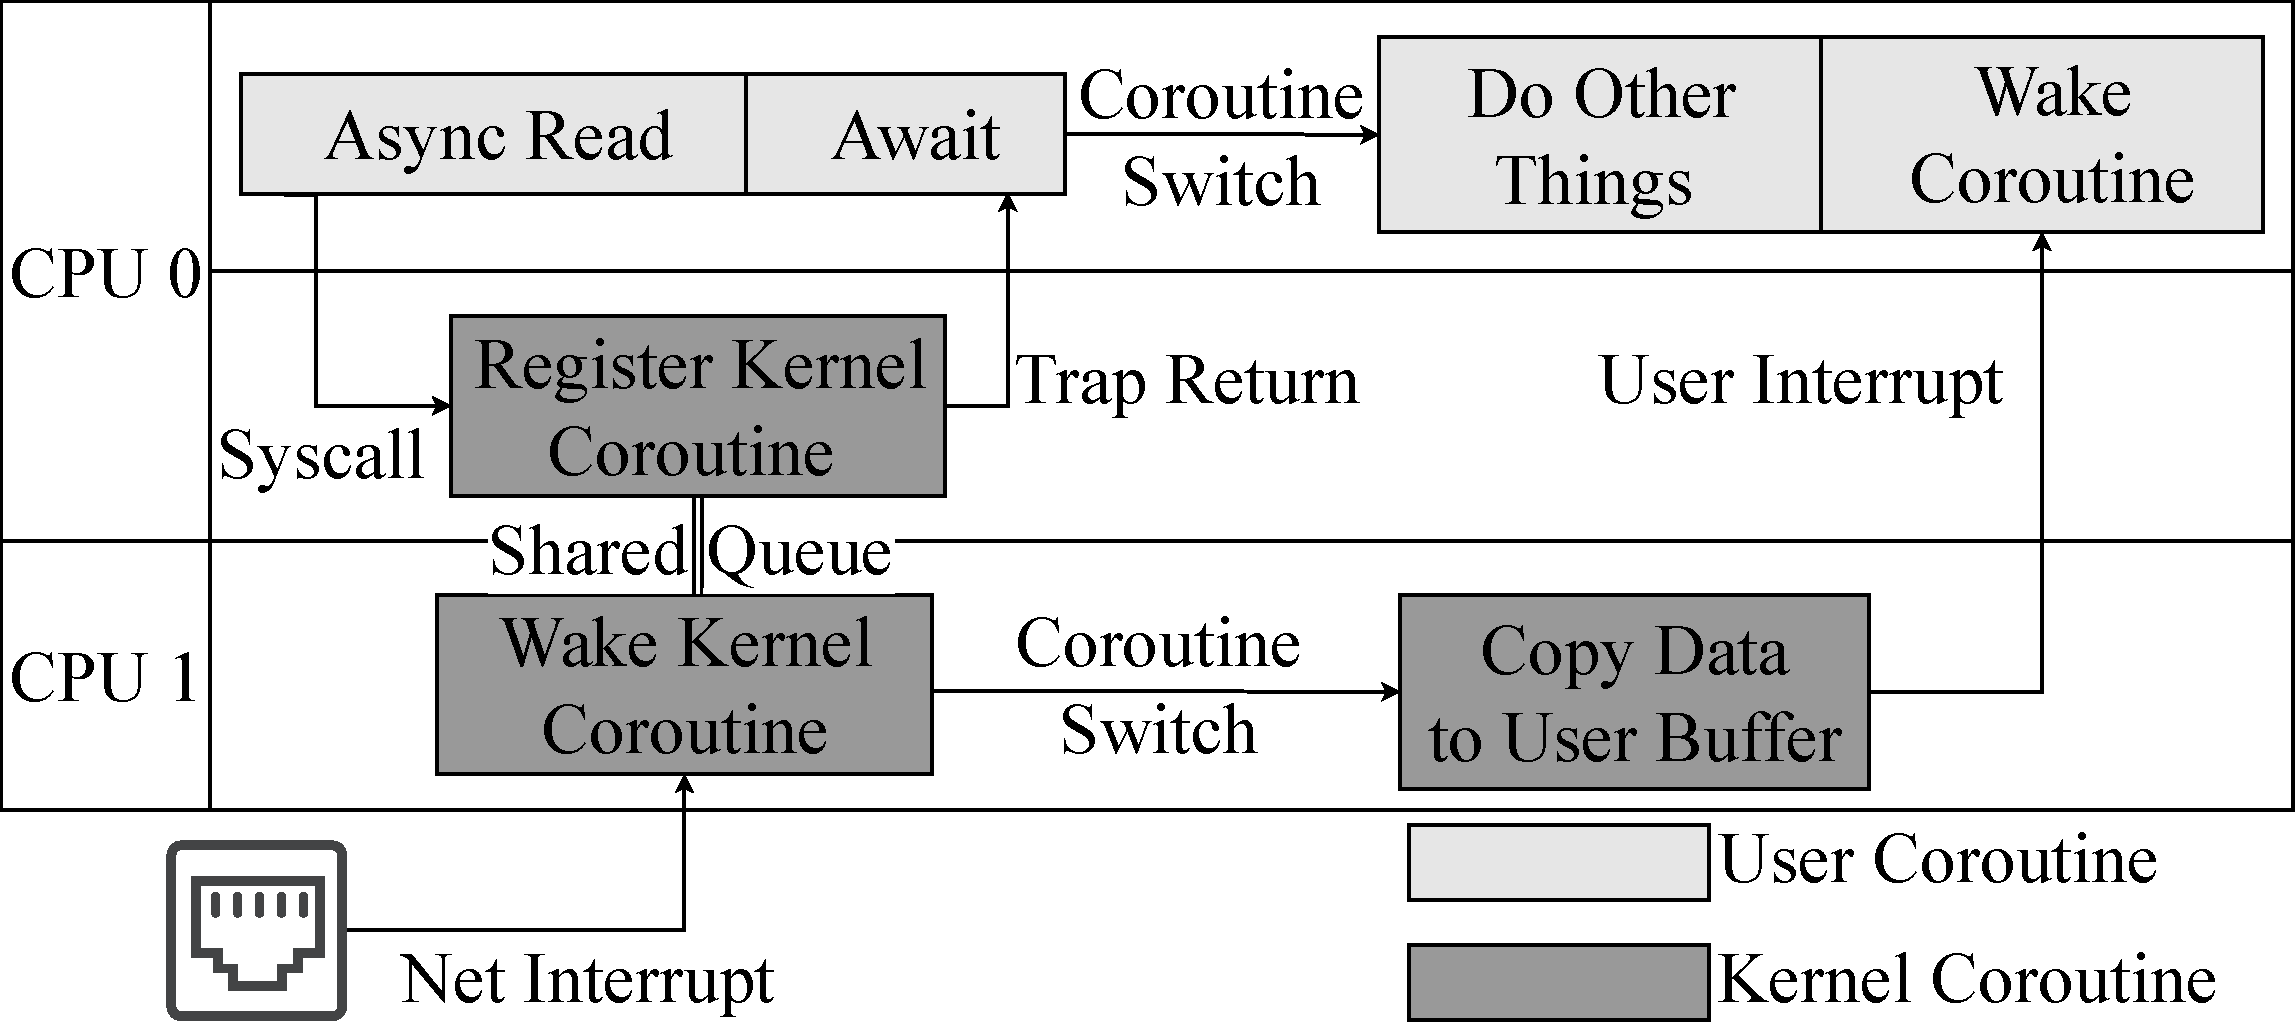
\includegraphics[width=\linewidth]{assets/async_syscall.pdf}
  \caption{Asynchronous system call.}
  \label{fig:async_syscall}
  \vspace{-1em}
\end{figure}

To demonstrate how coroutines integrate with asynchronous I/O, consider the example of reading data from sockets asynchronously. When a read operation reaches the kernel, it is handled by a kernel coroutine, allowing the control flow to return to user space immediately. The current user coroutine is then blocked, waiting for the kernel to complete the read, while COPS switches to execute another user coroutine. The kernel coroutine may run on a different CPU. If the data is ready in the buffer, the kernel coroutine proceeds without waiting, leveraging multi-processor capabilities. If the data is not ready, the kernel coroutine waits for the network card to signal it. During this wait, other kernel coroutines can continue executing. Once the kernel detects the network card's interrupt and prepares the data, it awakens the corresponding kernel coroutine to finish the operation, such as copying data to a user-space buffer. Upon completion, the kernel sends a user-level interruption, which in turn wakes up the corresponding user coroutine.

\section{Performance Evaluation}
\label{section: Performance Evaluation}

To assess COPS's capability in creating highly concurrent asynchronous programs and its precise control over coroutines, we conducted an evaluation on an FPGA. We used the Zynq UltraScale+ XCZU15EG MPSoC model \cite{zynq} to construct a five-stage RISC-V pipeline processor based on the rocket-chip \cite{rocket-chip}, a RISC-V soft IP core. Implementing N extension \cite{waterman_volume_nodate} on rocket-chip facilitated user-level interrupt functions, essential for asynchronous system calls. We operated an OS designed with the COPS framework on the RISC-V subsystem and evaluated COPS by simulating real-world web server application scenarios. The complete configuration parameters are detailed in Table \ref{tab:cfg}.

\begin{table}[tbp]
  \centering
  \begin{tabular}{|c|c|c|}
    \hline
    \multirow{3}{*}[-0.5cm]{FPGA} & \multicolumn{2}{c|}{ \makecell{Zynq UltraScale+ XCZU15EG MPSoC \cite{zynq}}} \\                             \cline{2-3}
                          & \makecell{RISC-V \\ soft IP core} & \makecell{ rocket-chip \cite{rocket-chip} with N \\ extension, 4 Core, 100MHz } \\ \cline{2-3}
                          & \makecell{Ethernet \\ IP core} & \makecell{Xilinx AXI 1G/2.5G \\ Ethernet Subsystem (1Gbps) \cite{axi-eth} } \\ \cline{2-3}
    \hline
    \makecell{Operating \\ System} & \multicolumn{2}{c|}{ rCore-tutorial\cite{rcore-os/rCore-Tutorial-v3} } \\ \cline{2-3}
                            
    \hline
    \makecell{Network \\ Stack} & \multicolumn{2}{c|}{ smoltcp\cite{smoltcp} } \\
    \hline
  \end{tabular}
  \caption{Configuration of evaluation.}
  \label{tab:cfg}
  \vspace{-1em}
\end{table}

The simulated web server application scenario is divided into two parts: a client on the PC regularly sends matrix data of a certain length to the server and awaits the response; The server, hosted on the FPGA, integrates two usage patterns: it establishes a connection with the client, processes the received matrix data, and sends the results back. The server comprises three components:

\begin{enumerate}[leftmargin=*]
    \item A request receiver that takes client requests and queues them;
    \item A request handler that dequeues requests, performs matrix operations, and queues the results;
    \item A response sender that retrieves responses from the queue and communicates them to the client.
\end{enumerate}

The PC client measures the latency of each request-response cycle and calculates the message throughput over a set time period. We assess COPS's performance by examining the web server's latency and throughput under various configurations.

\subsection{Coroutine vs. Thread}

To demonstrate the coroutine model's suitability for large-scale concurrency, we implemented the kernel and the web server's three components respectively using coroutines and threads\footnote{The threads in the application are kernel-support thread.}. The coroutine model assigns three coroutines per client-server connection, while the thread model assigns three threads per connection, each handling a component. We defined four server models based on the use of coroutines(\textbf{C}) and threads(\textbf{T}) in the kernel(\textbf{K}) and userland(\textbf{U}):

\textbf{KCUC}: When a user coroutine calls read(), the kernel creates a coroutine to perform the operation, blocking the user coroutine. Once data is read and copied, the kernel coroutine triggers a user-level interrupt to awaken the user coroutine.

\textbf{KCUT}: Similar to KCUC, but with a user thread invoking read(). The kernel coroutine executes the operation and unblocks the user thread after the copy is complete.

\textbf{KTUT}: A user thread calls read(), and a corresponding kernel thread reads data from the socket, blocking until the copy operation is done, allowing other threads to run in the meantime.
	
\textbf{KTUC}: Similar to KCUC, but instead of the kernel coroutine handling the copy, it delegates the read operation to a separate kernel thread, which polls sockets for data and copies it. Once the copy is complete, it sends a user-level interrupt to awaken the user coroutine.

The testing begins once all client-server connections are set up to avoid the influence of creating coroutines/threads. The client sends requests at 100ms intervals for a total of 5 seconds, with each request containing a 15x15 matrix. The results of the experiment are depicted in Fig.\ref{fig:throughput-latency}.

\begin{figure}[tbp]
	\centering
	\subcaptionbox{Throughput\label{subfig:throughput}}[0.49\linewidth]
	{
		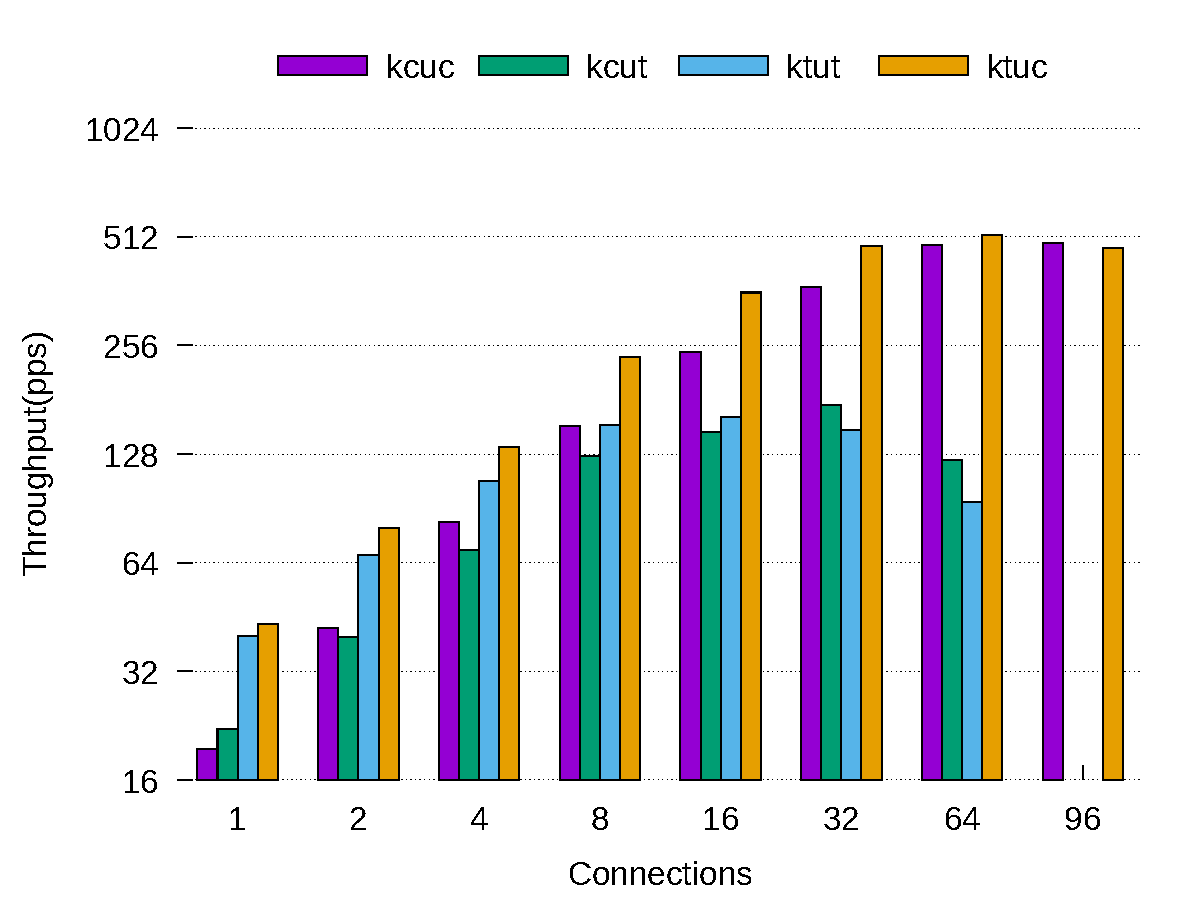
\includegraphics[width=\linewidth]{assets/throughput.pdf}
	}
	\subcaptionbox{Latency\label{subfig:latency}}[0.49\linewidth]
	{
		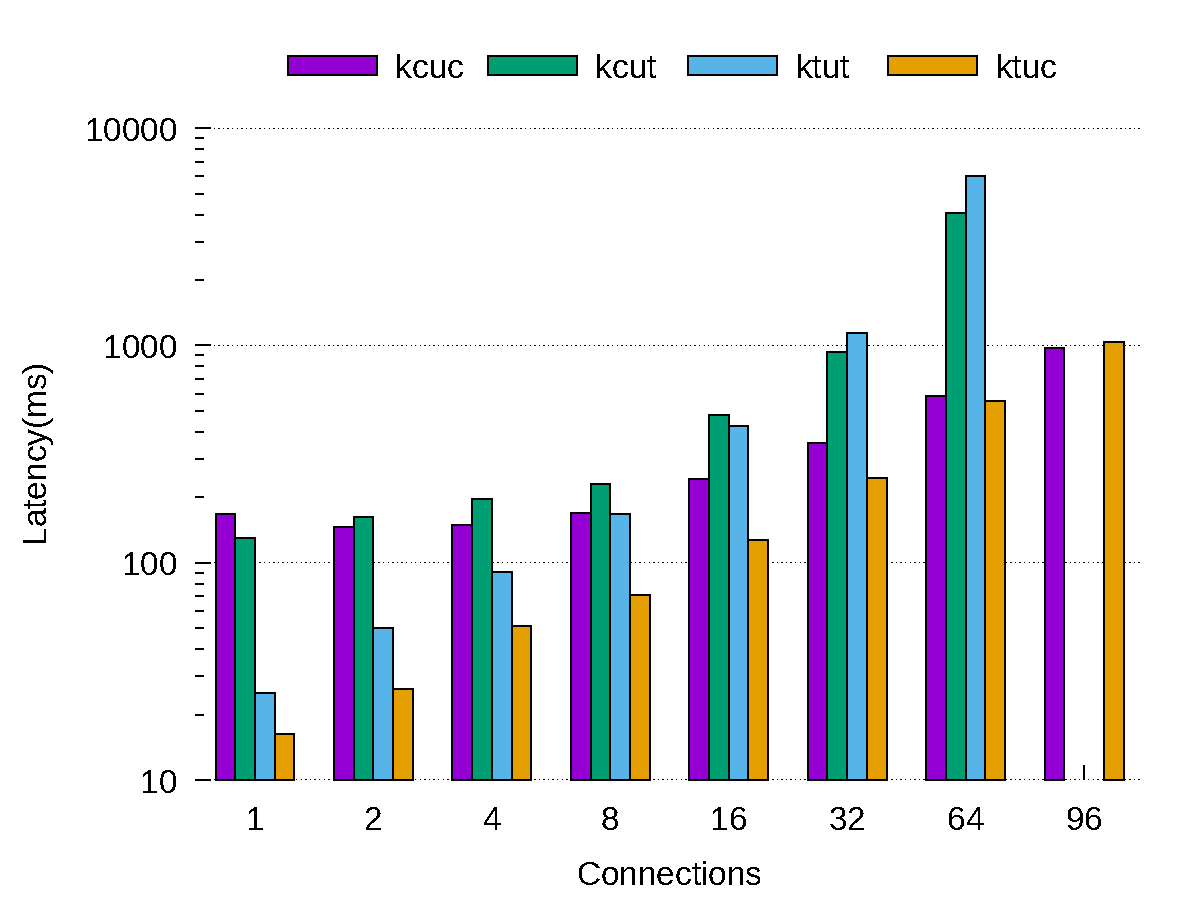
\includegraphics[width=\linewidth]{assets/latency.pdf}
	}
	\caption{Throughput and message latency.}
	\label{fig:throughput-latency}
  \vspace{-1em}
\end{figure}

\textbf{Runtime overhead}: With few connections, coroutines incur more overhead than threads, as seen in comparisons like KCUC vs KCUT, KCUT vs KTUT, and KCUC vs KTUT in Fig.\ref{fig:throughput-latency}. This overhead is due to COPS's executor being lock-protected. With a small number of connections, COPS can complete tasks with fewer cores but is given extra CPUs for a balanced comparison (the coroutine model has the same core allocation as the thread model). The extra CPUs lead to increased scheduling overhead from unnecessary synchronization. Additionally, frequent yielding on the extra core due to a lack of ready coroutines causes overhead from privilege level switching.

\textbf{Lower coroutine context-switching overhead}: As the number of connections grows, the latency of the thread model (KCUT and KTUT) exceeds that of the coroutine model (KCUC). By the time connections hit 32, KCUT's latency is notably lower than KTUT's. Despite performing the same operations, coroutines have less context-switching overhead than threads, even when comparing to kernel threads with streamlined context switching. At two connections, KCUC's latency is lower than KCUT's due to most context switches happening in userland in the KCUC model, avoiding the privilege-switching overhead present in KCUT. However, as connections increase further, the throughput of KCUT and KTUT decreases, and their context-switching costs rise rapidly.

\textbf{Coroutines have obvious advantages with high concurrency}: With a small number of connections, the KTUC model exhibits the lowest latency due to its dedicated kernel thread that polls socket states efficiently, providing a quick response. However, this advantage diminishes as connection numbers grow, and the KTUC model's polling overhead increases. Comparing throughput, at 64 connections, the CPU is fully loaded. At 96 connections, the KCUC model shows lower latency than KTUC, as the latter, along with KCUT and KTUT models, cannot complete the test due to the heavy workload. The specific throughput and message latency are not displayed in Fig.\ref{fig:throughput-latency} for these cases. As connections continue to increase, KTUC's throughput drops significantly, whereas KCUC's throughput remains relatively stable. Even with the use of epoll, which was not part of our experiment, the KTUC model's performance is unlikely to improve significantly due to additional synchronization overhead from its producer-consumer model and increased thread context-switching costs. In conclusion, after comparing KCUC with KTUC, COPS proves more suitable for large-scale concurrent scenarios.

\textbf{Less memory usage}: We also compared the memory usage between coroutines and threads. User-level threads, supported by the kernel, have two stacks: one for userland execution and another for kernel execution. In contrast, both kernel and userland coroutines run on a single stack, statically sized at 0x4000 bytes. The memory footprint of the three components using coroutines is as follows: 120 bytes for the request receiver, 80 bytes for the request handler, and 64 bytes for the response sender. The kernel coroutine itself is 176 bytes. Thus, establishing a connection in the KTUT model requires 0x4000 * 2 * 3 bytes, while the KCUC model requires only 0x4000 * 2 + 176 + 120 + 80 + 64 bytes. Table \ref{tab:mem_usage} illustrates the maximum number of connections possible for both the KTUT and KCUC models under specific configurations.

\begin{table}[htbp]
  \centering
  \begin{tabular}{cccc}
    \hline
    Configuration & Size(bytes) & KCUC & KTUT \\ \hline
    kernel heap   & 0x80\_0000  & \multirow{3}{*}{385} & \multirow{3}{*}{186} \\ 
    kernel frame  & 0x1A0\_0000  \\ 
    user heap     & 0x20\_0000   \\ 
    \hline
  \end{tabular}
  \caption{Maximum connections of KCUC and KTUT.\textnormal{The stack used by the thread is allocated from the kernel frame.}}
  \label{tab:mem_usage}
  \vspace{-1em}
\end{table}

\subsection{Priority orientation}

In a realistic scenario, a web server may manage tens of thousands of connections, many of which could be idle. System resources should favor active connections, prioritizing timely responses for them. We assign each connection a priority level in a tiered structure to ensure that higher-priority connections experience lower latency and less latency variability.

Similar to the previous experiment, but with both the kernel and application using coroutines. We establish 64 client-server connections with an equal distribution across 8 priority levels and measure throughput and message latency for each priority during the same time frame. The client sends requests to the server every 50ms over 5 seconds.

As shown in Fig.\ref{fig:prio-throughput-latency}, under limited resources, the throughput and latency for higher-priority connections are maintained. As resource availability increases(increasing the amount of CPU), lower-priority connections also see improved throughput and reduced latency, while the highest-priority connections consistently achieve the highest throughput and lowest latency.

\begin{figure}[tbp]
	\centering
	\subcaptionbox{Throughput\label{subfig:prio-throughput}}[0.49\linewidth]
	{
		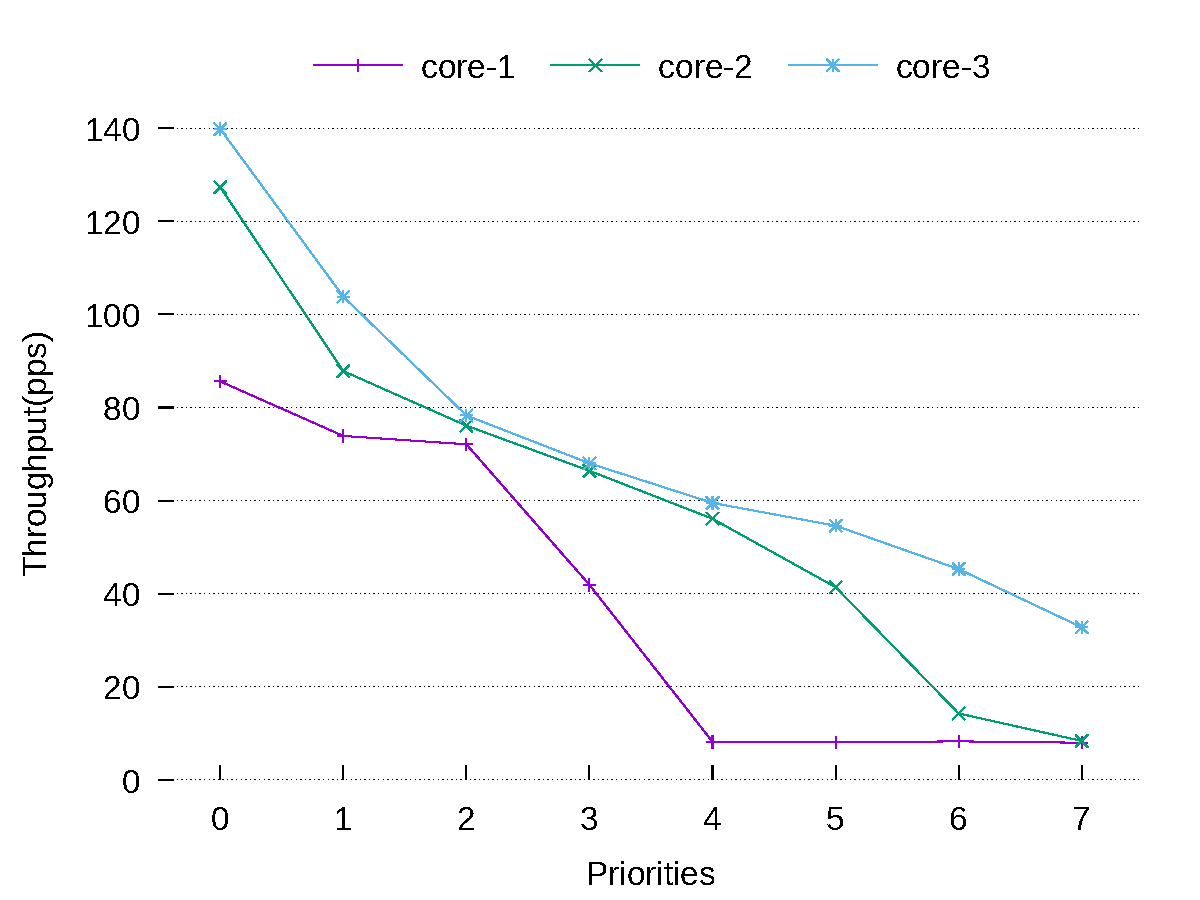
\includegraphics[width=\linewidth]{assets/prio-throughput.pdf}
	}
	\subcaptionbox{Latency\label{subfig:prio-latency}}[0.49\linewidth]
	{
		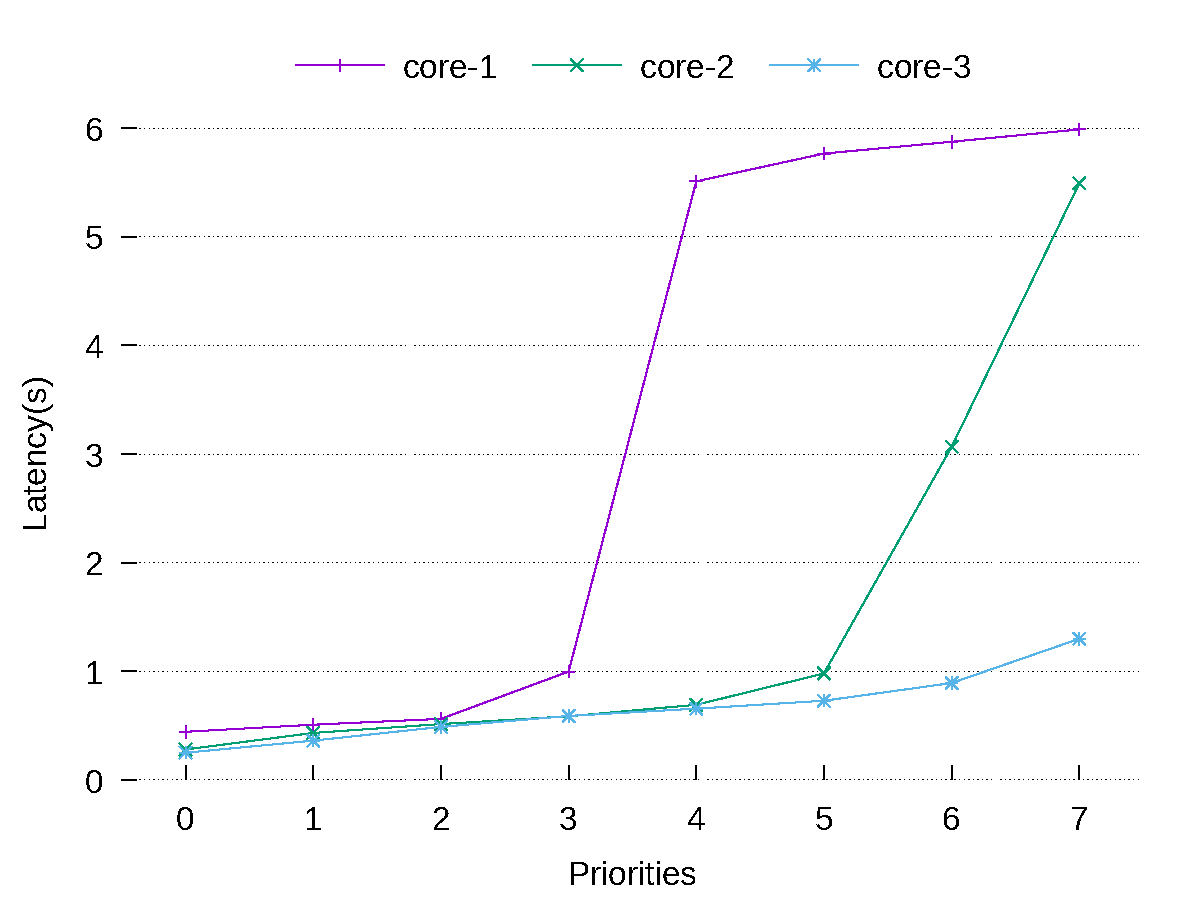
\includegraphics[width=\linewidth]{assets/prio-latency.pdf}
	}
	\caption{Throughput and message latency of different priority connections.}
	\label{fig:prio-throughput-latency}
	\vspace{-1.0em}
\end{figure}

Additionally, we created 64 connections between the client and server, evenly spread across 4 priority levels, to analyze the latency distribution for each priority. The results are depicted in Fig.\ref{fig:prio-cores}. Consistent with priority handling, higher-priority connections exhibit concentrated and low latency, whereas lower-priority connections show dispersed and higher latency. As resources increase, latency across all priorities decreases and becomes more concentrated.

\begin{figure}[tbp]
    \centering
    \subcaptionbox{Core-2\label{subfig:prio-core2}}[0.49\linewidth]
    {
      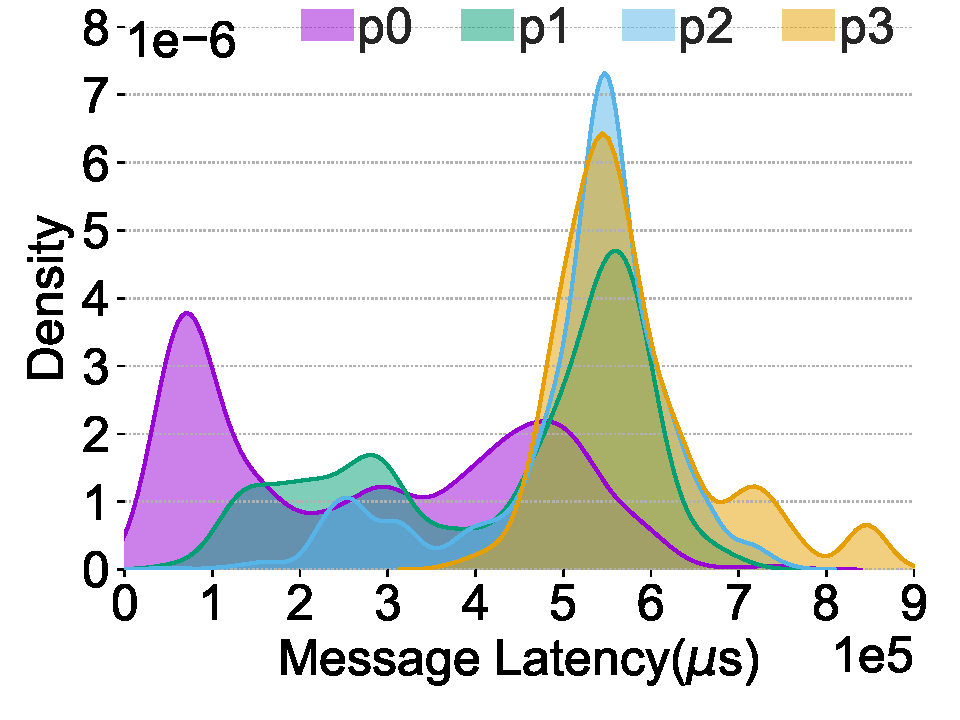
\includegraphics[width=\linewidth]{assets/prio-core2.pdf}
    }
    \subcaptionbox{Core-4\label{subfig:prio-core4}}[0.49\linewidth]
    {
      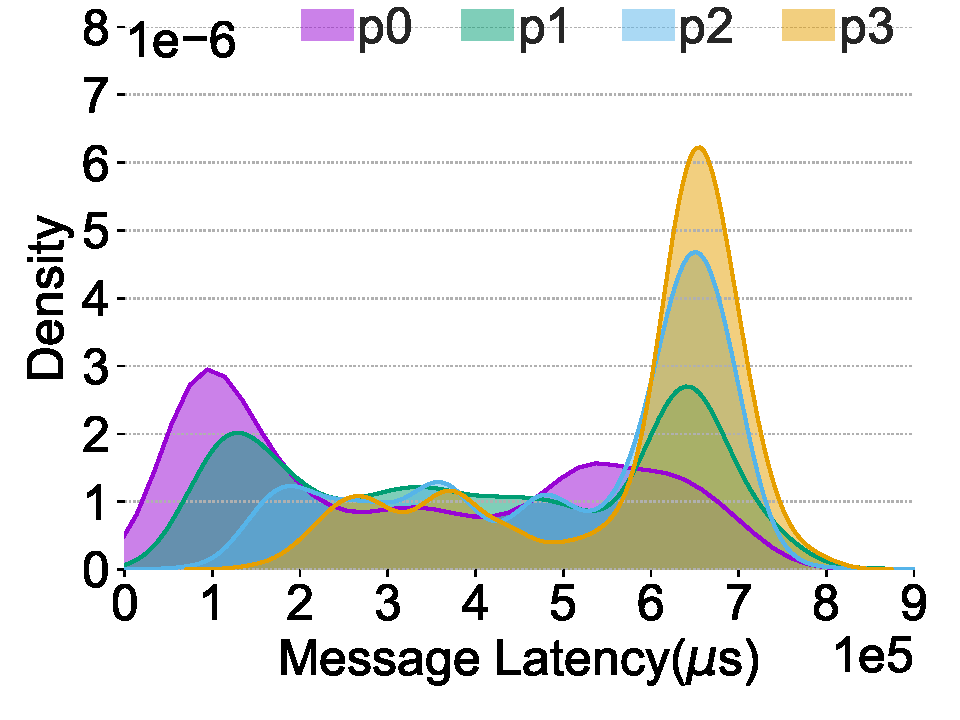
\includegraphics[width=\linewidth]{assets/prio-core4.pdf}
    }
    \caption{Latency distribution of different priority connections in different amount of cores.}
    \label{fig:prio-cores}
    \vspace{-1em}
\end{figure}

\section{Related Work}
\label{section: Related Work}

Coroutines, being lightweight with efficient context switching, are well-suited for the event-driven, state-machine approach often used in I/O operations. This has led to a surge in research leveraging coroutines.

Demikernel\cite{zhang_demikernel_2021} utilizes Rust coroutines to construct a system prototype, bypassing the overhead of context switches in I/O stacks, which typically take about 12 cycles. Their TCP stack assigns a coroutine per TCP connection for retransmissions, maintaining TCP state locally and eliminating the need for global state management, resulting in microsecond-level latency.

Embassy\cite{embassy}, an asynchronous driver framework for embedded systems built on Rust coroutines, excels in managing device interrupts. It significantly outperforms FreeRTOS, a C-based system, in interrupt handling time, thread processing time, and interrupt latency.

\section{Conclusion}
\label{section: Conclusion}

This paper introduces COPS, a coroutine-based priority scheduling framework, which allows the operating system to perceive user-level coroutines through a priority bitmap mechanism. COPS integrates coroutines with asynchronous I/O mechanisms, thereby facilitating the development of highly concurrent applications, reducing the overhead of traditional multi-threading, and providing efficient asynchronous I/O and priority scheduling.

Our evaluation demonstrates COPS's ability to deliver high throughput and low latency for highly concurrent applications. Compared to threads (KCUC vs KTUT), COPS's coroutine abstraction can increase throughput by 1.05 to 3.93 times. Additionally, COPS's coroutine priority scheduling effectively meets various requirements and ensures the rational distribution of system resources.

\bibliographystyle{IEEEtran}
\bibliography{IEEEabrv,refs}

\end{document}
